\section{Operationsverstärker \formelbuch{3}}
		\subsection{Opamp Schaltungen}
		\subsubsection{Invertierender Verstärker \formelbuch{3-7}}
			\begin{minipage}[T]{12cm}
          	  Bein invertierenden Verstärker ist die Ausgangsspannung gegenphasig
            	zur Eingangsspannung.\\
            	Closed-Loop Spannung:
            	\hspace{23mm}\fbox{$A_{CL}=\frac{v_{out}}{v_{in}}=-
            	\frac{R_F}{R_1}$}\\
            	\hspace*{10mm}\fbox{$i_1=\frac{v_{in}+v_d}{R_1}$}
           		\hspace{29.5mm}\fbox{$i_F=-\frac{v_{out}+v_d}{R_F}$}\\
            	Ausgangswiderstand des I-Verstärkers: \fbox{$r_{out}=0\Omega$}\\
            	Eingangswiderstand des I-Verstärkers:
            	\hspace{0.5mm}\fbox{$r_{in}=R_1$}
            \end{minipage}
			\begin{minipage}{6cm}
            	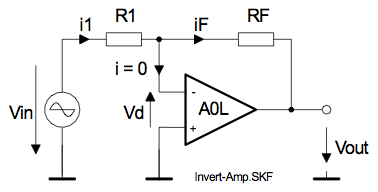
\includegraphics[width=6cm]{./bilder/i-verstaerker.png}
            \end{minipage}\\

\hrule

		\subsubsection{Nichtinvertierender Verstärker \formelbuch{3-10}}
			\begin{minipage}[T]{12cm}
            	Bein nichtinvertierenden Verstärker ist die Ausgangsspannung
            	gleichphasig zur Eingangsspannung.\\ Closed-Loop Gain:
            	\hspace{32mm}
            	\fbox{$A_{CL}=\frac{v_{out}}{v_{in}}=\frac{R_F}{R_1}+1$}\\
            	\hspace*{10mm}\fbox{$i_1=\frac{v_{in}-v_d}{R_1}$}
            	\hspace{32mm}\fbox{$i_F=\frac{v_{out}}{R_F+R_1}$}\\
            	Ausgangswiderstand des NI-Verstärkers: \fbox{$r_{out}=0\Omega$}\\
            	Eingangswiderstand des NI-Verstärkers:
            	\hspace{1mm}\fbox{$r_{in}=\infty$}
            \end{minipage}
			\begin{minipage}{6cm}
            	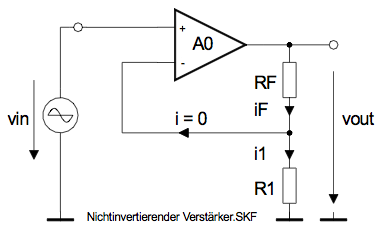
\includegraphics[width=6cm]{./bilder/ni-verstaerker.png}
            \end{minipage}\\

\hrule

		\subsubsection{Verstärker mit mehreren Eingängen \formelbuch{3-12}}
			\begin{minipage}{12.5cm}
            	\hspace*{10mm}\fbox{$A_{CL1}=-\frac{R_F}{R_1}$}
            	\hspace{15mm}\fbox{$A_{CL2}=-\frac{R_F}{R_2}$}\\
            	\hspace*{10mm}\fbox{$A_{CL3}=\frac{R_F+(R_1//R_2)}{(R_1//R_2)}$}\\
            	\hspace*{10mm}\fbox{$v_{out}=A_{CL1}v_1+A_{CL2}v_2+A_{CL3}v_3=
            	-\frac{R_F}{R_1}v_1-\frac{R_F}{R_2}v_2+\frac{R_F+(R_1//R_2)}{(R_1//R_2)}$}
            \end{minipage}
			\begin{minipage}{5.5cm}
            	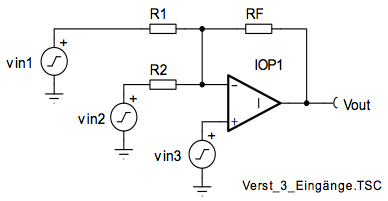
\includegraphics[width=5.5cm]{./bilder/3-eingaenge.png}
            \end{minipage}\\

\hrule

		\subsubsection{Invertierender Addierer \formelbuch{3-20}}
			\begin{minipage}[b]{12cm}
            \hspace*{10mm}\fbox{$V_{out}=A_{CL1}V_{IN1}+A_{CL2}V_{IN2}+\ldots$}\\
            \hspace*{10mm}\fbox{$A_{CL1}=- \frac{R_F}{R_1}$}
           	\hspace*{10mm}\fbox{$A_{CL2}=- \frac{R_F}{R_2}$}
            \end{minipage}
			\begin{minipage}{6cm}
            	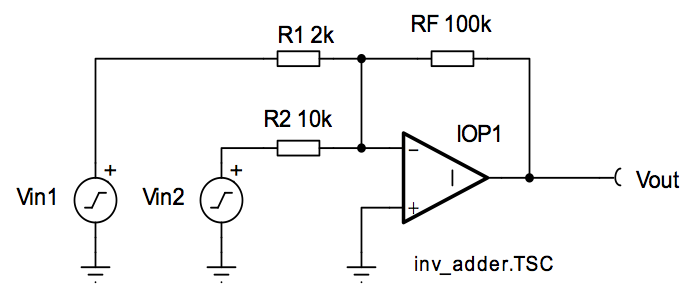
\includegraphics[width=6cm]{./bilder/invertadd.png}
            \end{minipage}\\

\hrule

		\subsubsection{Gewichteter Subtrahierer \formelbuch{3-20}}
			\begin{minipage}[b]{12cm}
            	\hspace*{10mm}\fbox{$A_{CL1}=- \frac{R_F}{R_1}$}\\
            	\hspace*{10mm}\fbox{$A_{CL2}=
           		\frac{R_3}{R_3+R_2}\left(1+\frac{R_F}{R_1}\right)$}\\
            	\hspace*{10mm}\fbox{$v_{out}=
            	\frac{R_3}{R_3+R_2}\left(1+\frac{R_F}{R_1}\right)
            	v_{in2}-\frac{R_F}{R_1}v_{in1}$}
            \end{minipage}
			\begin{minipage}{6cm}
            	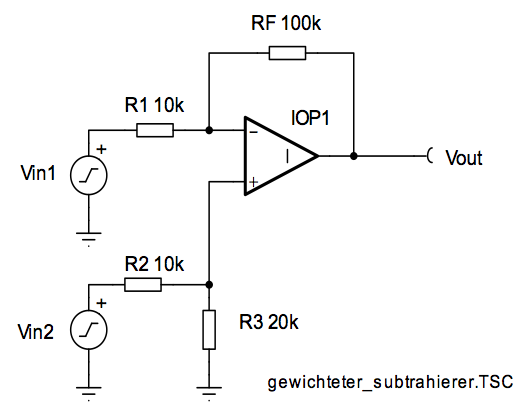
\includegraphics[width=6cm]{./bilder/gewichtsub.png}
            \end{minipage}\\
\newpage


		\subsubsection{Mehrfach-Addierer-Subtrahierer \formelbuch{3-23}} 		
		\begin{minipage}[b]{12cm}
		1. Man waehlt $R_{F}$\\
		2. Man waehlt $R_{P}$, wobei oft $R_{P}=R_{F}$ gesetzt wird. (optional)\\
		3. $R_{n}=\frac{R_{F}}{\left|A_{n}\right|}$ oder
			$R_{n}=\frac{R_{P}}{\left|A_{n}\right|}$\\ 
		4. Verstärkungsbedingung: $A_{N1} +
		\ldots + A_{Nn} = A_{P1} + \ldots + A_{Pn}$ \\Falls unerfüllt, muss ein Dummyeingang hinzugefügt werden!
		\end{minipage}
		\begin{minipage}{6cm}
          	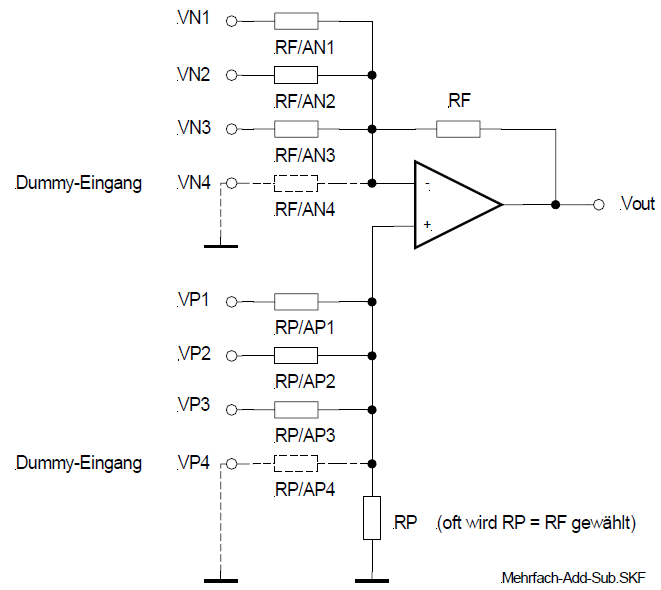
\includegraphics[width=6cm]{./bilder/mehrfach-addierer-subtrahierer.png} 
        \end{minipage}\\
		
		
\hrule

		\subsubsection{Instrumentenverstärker \formelbuch{3-25}}
		\begin{minipage}[b]{12cm}
		\hspace*{10mm}\fbox{$A_{diff}=\frac{V_{out}}{V_{diff}}=\frac{V_{P}-V_{N}}{V_{inP}-V_{inN}}
		=\frac{2R_{1}+P}{P}=\frac{2R_{1}}{P}+1$}\\
		\end{minipage}
		\begin{minipage}{6cm}
          	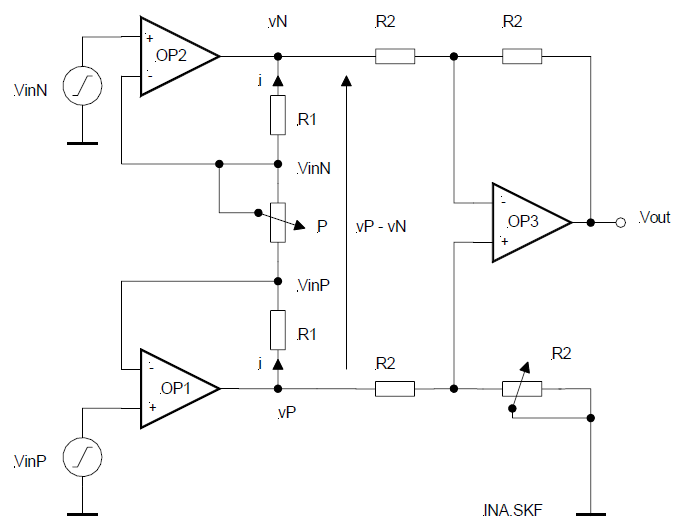
\includegraphics[width=6cm]{./bilder/Instrumentationsverstaerker.png} 
        \end{minipage}\\
		
\hrule

		\subsubsection{Differenzverstärker \formelbuch{3-21}}
			\begin{minipage}[b]{12cm}
            	\hspace*{10mm}\fbox{$A_{diff}=\frac{v_{out}}{(v_{in2}-v_{in1})}$}\\
            	\\ Widerstandsbedingung für den Differenzverstärker\\ \\
            	\hspace*{10mm}\fbox{$\frac{R_F}{R_1}=\frac{R_3}{R_2}$}
            	\hspace{15mm}\fbox{$A_{diff}=\frac{R_F}{R_1}=\frac{R_3}{R_2}$}
            	\hfill
            \end{minipage}
			\begin{minipage}{6cm}
            	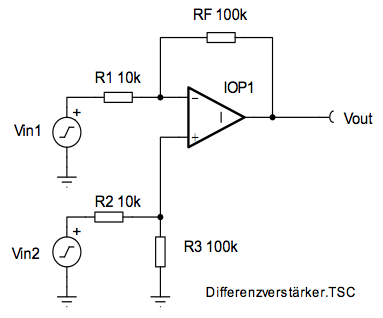
\includegraphics[width=6cm]{./bilder/differenzver.png}
            \end{minipage}\\

\newpage

		\subsubsection{Komparatorschaltung \formelbuch{3-27}}
			\begin{minipage}{18cm}
            	Wenn ein Operationsverstärker als {\it Verstärker ohne
            	Gegenkopplung} betrieben wird, spricht man von einer {\it
            	Komparatorschaltung}. Der Operationsverstärker wird dann als {\it
            	Komparator} betrieben.\\
            	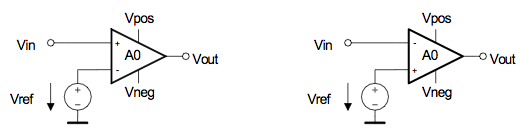
\includegraphics[width=16cm]{./bilder/komparator.png}\\
            	Beim nichtinvertierenden Komparator (links)\\
            	\hspace*{10mm}\fbox{$V_{out}=V_{out\hspace{1mm}max}=V_{pos}-V_{Rand}
            	\mbox{ wenn } V_{in} > V_{ref}\pm V_{OS} \mbox{ bzw. } 
            	V_{diff}\pm V_{OS}>0$}\\
            	\hspace*{10mm}\fbox{$V_{out}=V_{out\hspace{1mm}min}=V_{neg}+V_{Rand}
            	\mbox{ wenn } V_{in} < V_{ref}\pm V_{OS} \mbox{ bzw. } 
            	V_{diff}\pm V_{OS}<0$}\\ \\
            	Beim invertierenden Komparator (rechts)\\
            	\hspace*{10mm}\fbox{$V_{out}=V_{out\hspace{1mm}max}=V_{pos}-V_{Rand}
            	\mbox{ wenn } V_{in} < V_{ref}\pm V_{OS} \mbox{ bzw. } 
            	V_{diff}\pm V_{OS}<0$}\\
            	\hspace*{10mm}\fbox{$V_{out}=V_{out\hspace{1mm}min}=V_{neg}+V_{Rand}
            	\mbox{ wenn } V_{in} > V_{ref}\pm V_{OS} \mbox{ bzw. } 
            	V_{diff}\pm V_{OS}>0$}\\
            \end{minipage}

\hrule
		
		\subsubsection{Schmitt-Trigger \formelbuch{3-31}}
		Nichtinvertierender Schmitt-Trigger\\
			\begin{minipage}{9cm}
	          	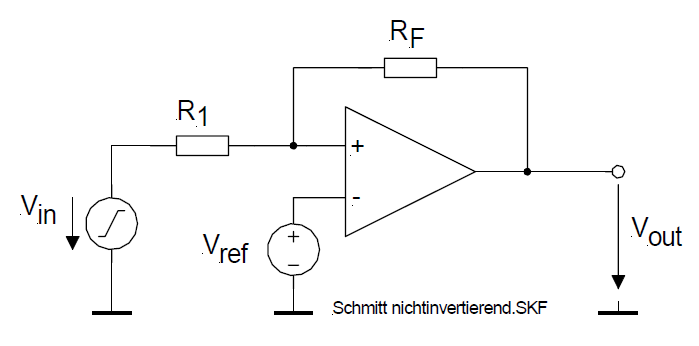
\includegraphics[width=8cm]{./bilder/n-schmitt.png} 
	        \end{minipage}
			\begin{minipage}{9cm}
	          	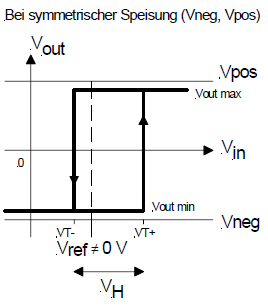
\includegraphics[width=4cm]{./bilder/n-schmitt-kennlinie.png} 
	        \end{minipage}\\
		Invertierender Schmitt-Trigger\\
			\begin{minipage}{9cm}
	          	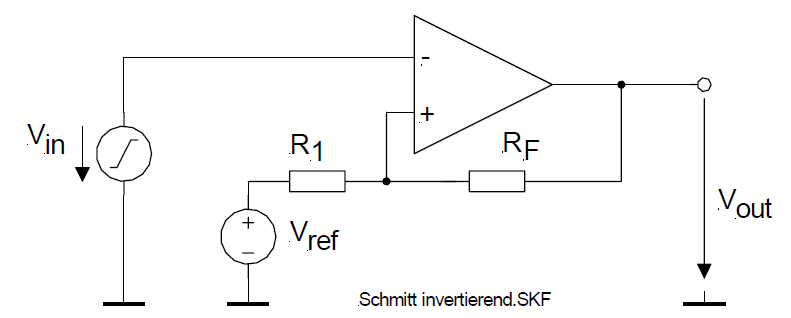
\includegraphics[width=8cm]{./bilder/i-schmitt.png} 
	        \end{minipage}
			\begin{minipage}{9cm}
	          	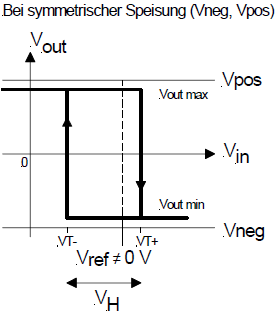
\includegraphics[width=4cm]{./bilder/i-schmitt-kennlinie.png} 
	        \end{minipage}\\
			
			\begin{minipage}{18cm}
               	Hysteresespannung:\\
               	\hspace*{10mm}
               	\begin{tabular}{| c | c |}
                \hline
                Nichtinvertierender Schmitt-Trigger & Invertierender
                Schmitt-Trigger\\
                \hline
                $V_H=(V_{out \hspace{1mm} max}-V_{out \hspace{1mm}
                min})\frac{R_1}{R_F}$ &
                $V_H=(V_{out \hspace{1mm} max}-V_{out \hspace{1mm}
                min})\frac{R_1}{R_1+R_F}$\\
                \hline
            \end{tabular}\\ \\
				Schwellspannung:\\
				\hspace*{10mm}
			\begin{tabular}{| c | c |}
                \hline
                Nichtinvertierender Schmitt-Trigger & Invertierender
                Schmitt-Trigger\\
                \hline
                $V_{T+}=V_{ref}+(V_{ref}-V_{out
                \hspace{1mm} min})\frac{R_1}{R_F}$ &
                $V_{T+}=V_{ref}+(V_{out \hspace{1mm}
                max}-V_{ref})\frac{R_1}{R_1+R_F}$\\
                \hline
                $V_{T-}=V_{ref}-(V_{out
                \hspace{1mm} max}-V_{ref})\frac{R_1}{R_F}$ &
                $V_{T-}=V_{ref}-(V_{ref}-V_{out \hspace{1mm}
                min})\frac{R_1}{R_1+R_F}$\\
                \hline
            \end{tabular}\\
            \end{minipage}

\newpage
	
		\subsubsection{Differentiator \formelbuch{3-42}}
			\begin{minipage}[b]{12cm}
           		Beim Differentiator gilt $v_{out}=v_N-i_1 \cdot R_F$ wobei
           		$v_N=0$\\ \hspace*{10mm}\fbox{$i_1=C_1 \cdot \frac{dv_C}{dt}$}\\
           		\hspace*{10mm}\fbox{$v_{out}=-R_FC_1 \frac{dv_{in}}{dt}$}\\
           		Die Elemente $C_F$ und $R_1$ sind optional. \\
           		Sie beheben jedoch Probleme die ohne \\
           		sie entstehen (siehe elemenarer Differentieator). \\
           		Mit $C_F$ und $R_1$: \\
           		- Keine differentiation bei hoeheren Frequenzen. \\
           		- Limitierte Verstaerkuing bei hoeheren Frequenzen. \\
           		- Eingangswiderstand immer groesser $R_1$ \\ 
           		$\rightarrow$ keine Belastung der Signalquelle
           
           	\end{minipage}
			\begin{minipage}{6cm}
           		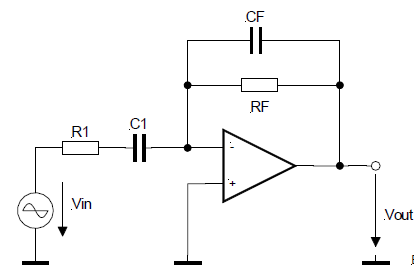
\includegraphics[width=6cm]{./bilder/differentiator.png}
           	\end{minipage}

\hrule

		\subsubsection{Integrator \formelbuch{3-45}} 
		\vspace{1cm}
		\begin{minipage}[b]{12cm}
		\hspace{8mm} \fbox{$v_{out}=-\frac{1}{RC} \int{v_{in}}dt +
		v_{out\hspace{1mm}Anfang} $}\\
		\hspace{8mm} \fbox{$\frac{dv_{out}}{dt}=-\frac{v_{in}}{RC}$}\\
		\end{minipage} 
		\begin{minipage}{6cm}
          	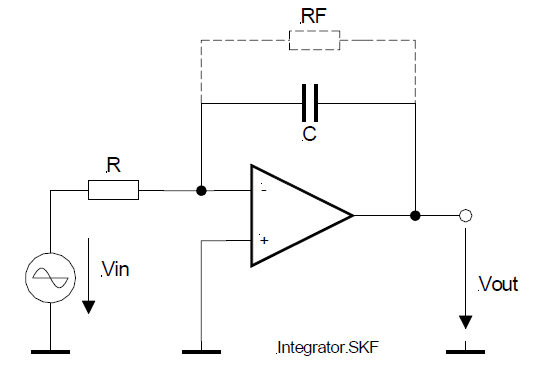
\includegraphics[width=6cm]{./bilder/integrator.png} 
        \end{minipage}\\
		
\hrule
		\subsection{Fehlereinflüsse des Opamp \formelbuch{3-51}}
		\subsubsection{Verstärkungsfehler bei endlicher Closed-Loop-Verstärkung
		\formelbuch{3-51}}
			\begin{minipage}{12cm}
               	beim nichtinvertierenden Verstärker 
               	\fbox{$A_{CL \hspace{1mm} ideal}=\frac{R_F}{R_1}+1$}\\
               	beim invertierenden Verstärker
               	\hspace{8mm}\fbox{$A_{CL \hspace{1mm}
               	ideal}=-\frac{R_F}{R_1}$}\\ \\
               	Beim invertierenden Verstärker ist eine kleine Korrektur
               	anzubringen: 
               	\hspace*{10mm}\fbox{$\frac{1}{A_{CL \hspace{1mm}
               	real}}=\frac{1}{A_{CL \hspace{1mm} real}}+\frac{1}{nA_{OL}}$}\\
	        \end{minipage}
			\begin{minipage}{6cm}
               	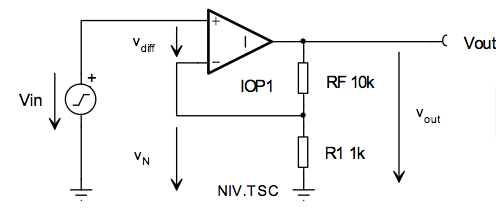
\includegraphics[width=6cm]{./bilder/verstaerkungsfaktor.png}
            \end{minipage}

\hrule

		\subsubsection{Common-Mode-Fehler \formelbuch{3-60}}
			\begin{minipage}{6cm}
            	Mittelspannung: \fbox{$V_M=\frac{V_{pos}+V_{neg}}{2}$}\\
            	Offsetspannung: \fbox{$V_{OS}=\frac{V_{CM}}{CMRR_{lin}}$}
            \end{minipage}
			\begin{minipage}{12cm}
            	Opamp-Eingangsspannung: \fbox{$V_{OP \hspace{1mm} IN}=\frac{V_P+V_N}{2}$}\\
            	Ausgangs-Fehlerspannung: \hspace{0.2mm}
            	\fbox{$V_{out \hspace{1mm} E}=\left|V_{OS}\right| \cdot A_{CL+}=\left| \frac{\Delta V_{CM}}{CMRR_{lin}}\right|A_{CL+}$}
            \end{minipage}

			\begin{minipage}{18cm}
            	Common-Mode-Spannung:
            	\fbox{$V_{CM}=V_{OP \hspace{1mm} IN}-V_M=V_P- \frac{V_{pos}+V_{neg}}{2} \mbox{ bzw. }V_N- \frac{V_{pos}+V_{neg}}{2}$}\\
            	\hspace*{4.2cm}\fbox{$V_{CM}\frac{V_{P}+V_{N}}{2}-V_M$}\\
            	Lineare Definition: \hspace{11mm}
            	\fbox{$CMRR_{lin}=\frac{dV_{CM}}{dV_{OS}}=10^{\frac{CMRR_{dB}}{20}}$}
            	\hspace{11mm}
            	\fbox{$CMRR_{lin}=\frac{A_{OL}}{A_{CM}}$}\\
            	Logarithmische Definition:
            	\fbox{$CMRR_{dB}=20 \cdot log(CMRR_{lin})=20 \cdot log\frac{dV_{CM}}{dV_{OS}}$}\\
            \end{minipage}

\newpage
		
		\subsubsection{Offsetspannungsfehler \formelbuch{3-53}}
			\begin{minipage}{18cm}
            	Im Closed-Loop-Betrieb ist die Ausgangs-Fehlerspannung:\hspace{6mm}
            	\fbox{$V_{out \hspace{1mm}E}=V_{OS}\left( 1+\frac{R_F}{R_1}
            	\right)$} allgemein: $V_{out \hspace{1mm}E}=V_{OS}
            	\cdot {A_{CL}}^{+}$\\
            	Im Open-Loop-Betrieb ist die Ausgangs-Fehlerspannung:\hspace{6mm}
            	\fbox{$V_{out \hspace{1mm}E}=V_{OS}
            	\cdot {A_{CL}}^{+}$}\\
            \end{minipage}

\hrule
		
		\subsubsection{Eingangsstromfehler \formelbuch{3-54}}
			\begin{minipage}{18cm}
              Wenn die Opamp-Eingangsströme gleich gross sind
              ($I_{N}=I_{P}$) und die Gleichstromwiderstände,
              die von jedem Opamp-Eingang nach Masse führen, 
              ebenfalls gleich gross gewählt werden, heben sich die
              Ausgangsspannungsfehler, die durch $I_{N}$ und $I_{P}$
              erzeugt werden, gegenseitig auf. \\
              Allgemeine Formel für den
              Eingangsstromfehler:
                \hspace{20mm}
                \fbox{$V_{out \hspace{1mm}E}=I_N R_F-R_2 I_P\left( 1+\frac{R_F}{R_1} \right)$}\\ Widerstandsbedingung für Eingangsstromkompensation: \hspace{7.5mm}
            	\fbox{$R_2=\frac{R_F R_1}{R_F+R_1}=R_F // R_1$}\\
            \end{minipage}\\
			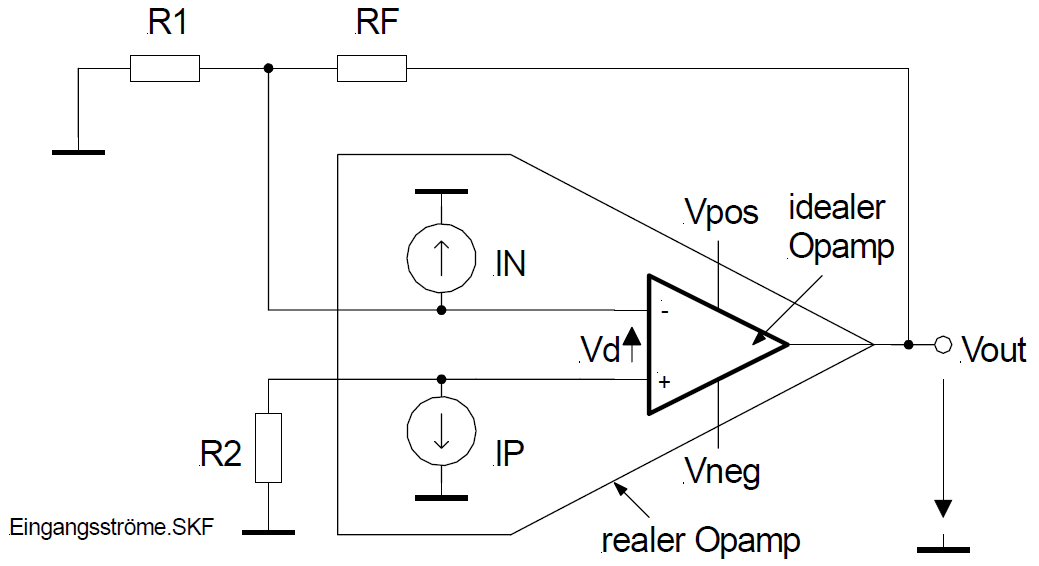
\includegraphics[width=8cm]{./bilder/eingangsstromfehler.png}


\hrule

		\subsubsection{Eingangsstromkompensation ohne AC-Zweige \formelbuch{3-54}}
			\begin{minipage}[b]{6cm}
            	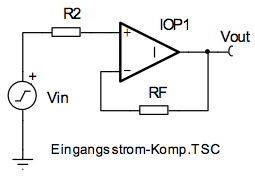
\includegraphics[height=3cm]{./bilder/spannungsfolger.png}\\
            	\centerline{{\bf Spannungsfolger}}\\ \\
            	$R_2$ sei ein gegebener Quellen-Widerstand\\
            	{\bf $R_F$ muss eingefügt werden}\\ \\
            	\fbox{$R_F=R_2$}
            \end{minipage}\hfill
			\begin{minipage}[b]{6cm}
            	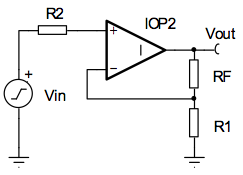
\includegraphics[height=3cm]{./bilder/nichtinver}\\
            	\centerline{{\bf Nichtinvertierender Verstärker}}\\ \\
            	Hier sei der Quellenwiderstand
            	vernachlässigbar.\\ {\bf $R_2$ muss eingefügt werden}\\ \\
            	\fbox{$R_2=R_F//R_1$}
            \end{minipage}\hfill
			\begin{minipage}[b]{6cm}
            	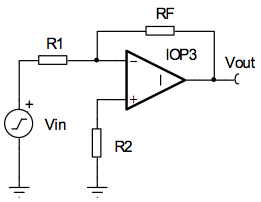
\includegraphics[height=3cm]{./bilder/inver}\\
            	\centerline{{\bf Invertierender Verstärker}}\\ \\ \\ \\
            	{\bf $R_2$ muss eingefügt werden}\\ \\
            	\fbox{$R_2=R_F//R_1$}
            \end{minipage}
			\begin{minipage}{18cm}
            	\vspace{3mm}
				\textbf{Ausgangsspannungsfehler} auf Grund des \textbf{Offsetstromes} (nur bei
				Kompensation(!)):
				\fbox{$V_{out \hspace{1mm}E}=\left|I_{OS}\right| \cdot R_F$}\\
			\end{minipage}
\hrule

		\subsubsection{Power-Supply-Fehler \formelbuch{3-58}}
			\begin{minipage}{18cm}
            Die grösse $PSRR$ (Power Supply Rejection Ratio, Speisespannungsunterdrückung)\\
            Offsetspannung: \fbox{$V_{OS}=\frac{\Delta V_{Supply}}{PSRR_{lin}}$}
            \hspace{10mm}
            Ausgangsspannungsfehler:
            \fbox{$V_{out \hspace{1mm}E}=\left|V_{OS}\right| A_{CL+}=\left| \frac{\Delta V_{Supply}}{PSRR_{lin}}\right| A_{CL+}$}\\
            Lineare Definition: \hspace{11mm}
            \fbox{$PSRR_{lin}=\frac{dV_{Supply}}{dV_{OS}}=10^{\frac{PSRR_{dB}}{20}}$}\\
            Logarithmische Definition:
            \fbox{$PSRR_{dB}=20 log PSRR_{lin}=20 log \frac{dV_{Supply}}{dV_{OS}}$}\\
            \end{minipage}

\hrule

		\subsubsection{Zusammenfassung aller Fehlereinflüsse \formelbuch{3-63}}
			\begin{minipage}{18cm}
            	\fbox{$V_{out\hspace{1mm}E\hspace{1mm}total}=A_{CL+}\cdot\left[\left|V_{OS}\right|+\frac{\left|V_{CM}\right|}{CMRR}
            	+\frac{\left|\Delta V_{Supply}\right|}{PSRR}\right]+\left|I_{OS}\right|R_F$}\\
            \end{minipage}

\newpage

		\subsection{Dynamische Eigenschaften des Opamp \formelbuch{3-66}}
			\begin{minipage}{18cm}
            	dB-Verstärkung: \hspace{4.5mm}
            	\fbox{$A_{dB}=20 \cdot log A_{lin}$}\\
            	lineare Verstärkung:
            	\fbox{$A_{lin}=10^{\frac{A_{dB}}{20}}$}\\ \\
            	Verstärkungs-Bandbreite-Produkt GBP (Gain-Bandwidth-Product)\\
            	Bandbreite des gegengekoppelten {\it nichtinvertierenden} Verstärkers:
            	\fbox{$f_{CL+}=\frac{GBP}{A_{CL \hspace{1mm}lin}}$}\\
            	Bandbreite des gegengekoppelten {\it invertierenden} Verstärkers: \hspace{6.5mm}
            	\fbox{$f_{CL}=\frac{GBP}{\left| A_{CL \hspace{1mm}lin}\right|+1}$}\\ \\
            	{\bf Gesetz vom Konstanten Verstärkungs-Bandbreite-Produkt:} \\ \\
            	Für jeden Punkt auf der mit -20dB abfallenden Frequenzgang-Gerade ist das
            	Produkt aus Verstärkung und zugehöriger Frequenz konstant gleich GBP, d.h. $A_{lin}\cdot f=GBP=konst$\\
            \end{minipage}
		\subsubsection{Slew-Rate}
		min. SR bei einem Sprungsignal \hspace{4mm}
		\fbox{$SR\geq\frac{0.8V_{step}}{t_{anstieg}}$}\\ 
		min. SR bei einem Sinussignal \hspace{4.5mm} 
		\fbox{$SR\geq V_{amplitude}\omega=V_{amplitude}2\pi f$}\\
		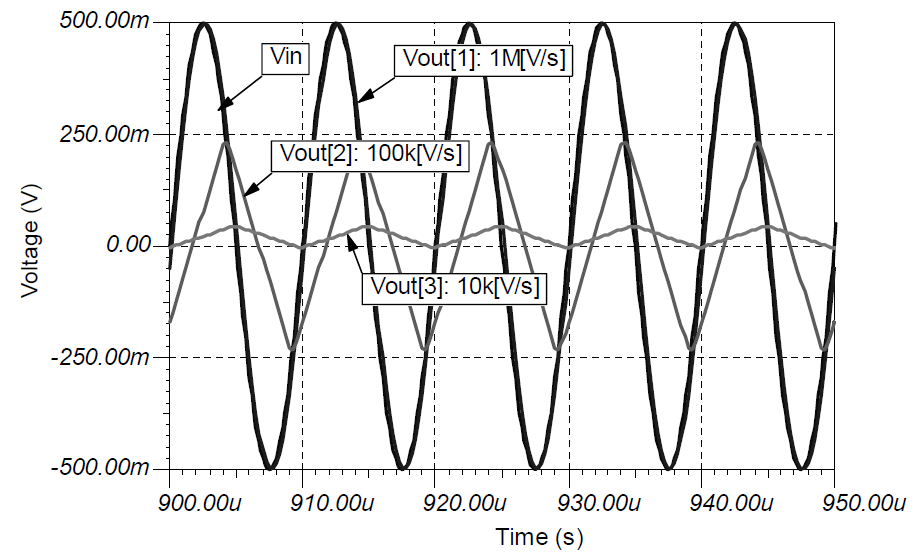
\includegraphics[height=5cm]{./bilder/slew-rate.png}\\